% TikZ figure: Sinusoidal positional encodings
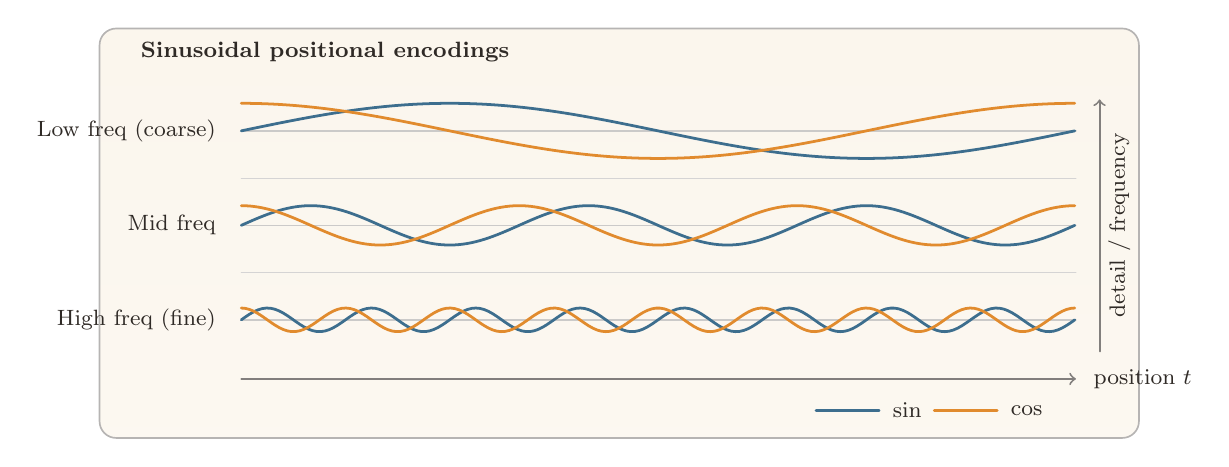
\begin{tikzpicture}[x=1cm,y=1cm, font=\small, line cap=round, line join=round]
  \definecolor{Ink}{HTML}{2F2A26}
  \definecolor{Panel}{HTML}{FBF6ED}
  \definecolor{WarmBlue}{HTML}{3D6E8E}
  \definecolor{WarmOrange}{HTML}{E18B2E}
  \definecolor{WarmGray}{HTML}{B9B1A8}

  \tikzset{
    panel/.style={rounded corners=6pt, draw=Ink!35, line width=0.6pt},
    note/.style={font=\footnotesize, text=Ink}
  }

  \def\xstart{1.2}
  \def\xwidth{10.6}
  \def\xscale{0.0294}

  \path[panel, shade, top color=Panel, bottom color=Panel!80] (-0.6,-0.9) rectangle (12.6,4.3);
  \node[note, anchor=west] at (-0.2,4.0) {\textbf{Sinusoidal positional encodings}};

  % Strips: low, mid, high frequency
  \draw[Ink!20, line width=0.4pt] (\xstart,2.4) -- (\xstart+\xwidth,2.4);
  \draw[Ink!20, line width=0.4pt] (\xstart,1.2) -- (\xstart+\xwidth,1.2);
  \foreach \y/\freq/\label/\amp in {
    3.0/1/Low freq (coarse)/0.35,
    1.8/3/Mid freq/0.25,
    0.6/8/High freq (fine)/0.15
  } {
    \node[note, anchor=east] at (1.0,\y) {\label};
    \draw[Ink!25, line width=0.5pt] (\xstart,\y) -- (\xstart+\xwidth,\y);
    \draw[WarmBlue, line width=1.0pt]
      plot[domain=0:360, samples=200] ({\xstart+\xscale*\x},{\y+\amp*sin(\freq*\x)});
    \draw[WarmOrange, line width=1.0pt]
      plot[domain=0:360, samples=200] ({\xstart+\xscale*\x},{\y+\amp*cos(\freq*\x)});
  }

  % Legend
  \draw[WarmBlue, line width=1.0pt] (8.5,-0.55) -- (9.3,-0.55);
  \node[note, anchor=west] at (9.35,-0.55) {sin};
  \draw[WarmOrange, line width=1.0pt] (10.0,-0.55) -- (10.8,-0.55);
  \node[note, anchor=west] at (10.85,-0.55) {cos};

  % Direction cues
  \draw[->, line width=0.7pt, draw=Ink!60] (1.2,-0.15) -- (11.8,-0.15);
  \node[note, anchor=west] at (11.9,-0.15) {position $t$};
  \draw[->, line width=0.7pt, draw=Ink!60] (12.1,0.2) -- (12.1,3.4);
  \node[note, rotate=90] at (12.35,1.8) {detail / frequency};
\end{tikzpicture}
